      
\begin{frame}[<+->]
\frametitle{Degree of Freedom Handling}

  \begin{block}{}
  \begin{itemize}
    \item{DofObject subclasses store global Degree of Freedom indices}
    \item{DofMap class assigns indices to a partitioned mesh}
    \item{FE classes calculate hanging node, periodic constraints}
    \item{DofMap class applies constraints}
    \item{System class handles AMR/C projections}
  \end{itemize}
  \end{block}
\end{frame}


\begin{frame}
\frametitle{Generic Constraint Calculations}

To maintain function space continuity, constrain ``hanging node''
Degrees of Freedom coefficients on fine elements in terms of DoFs on
coarse neighbors.

\begin{minipage}[h]{.45\textwidth}
  \begin{figure}[h]
    \begin{center}
      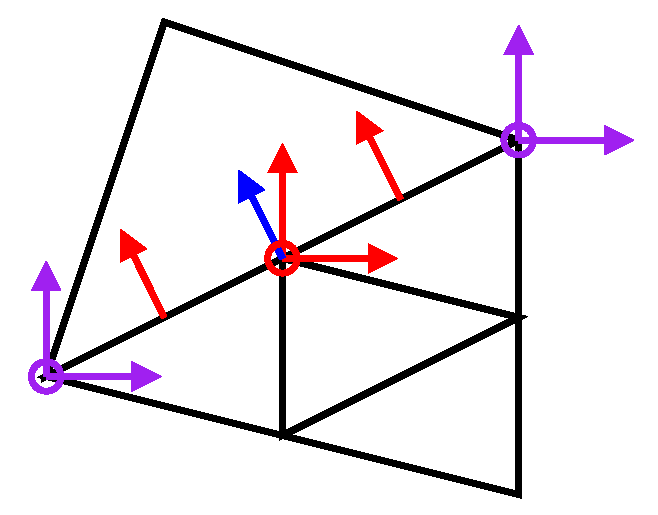
\includegraphics[width=.5\textwidth]{figs/hanging_node}
    \end{center}
  \end{figure}
\end{minipage}
\begin{minipage}[h]{.45\textwidth}
\begin{eqnarray*}
u^F & = & u^C \\
\sum_i u_i^F \phi_i^F & = & \sum_j u_j^C \phi_j^C \\
A_{ki} u_i & = & B_{kj} u_j \\
u_i & = & A_{ki}^{-1} B_{kj} u_j
\end{eqnarray*}
\end{minipage}

Integrated values (and fluxes, for $C^1$ continuity) give
element-independent matrices:
\begin{eqnarray*}
A_{ki} & \equiv & (\phi_i^F, \phi_k^F) \\
B_{kj} & \equiv & (\phi_j^C, \phi_k^F)
\end{eqnarray*}

\end{frame}



\begin{frame}
\frametitle{Generic Projection Calculations}

Upon element coarsening (or refinement in non-nested spaces):

  \begin{block}{}
  \begin{itemize}
    \item{Copy nodal Degree of Freedom coefficients}
    \item{Project edge DoFs, holding nodal DoFs constant}
    \item{Project face DoFs, holding nodes/edges constant}
    \item{Project interior DoFs, holding boundaries constant}
  \end{itemize}
  \end{block}

  \begin{block}{Advantages / Disadvantages}
  \begin{itemize}
    \item{Requires only local solves}
    \item{Consistent in parallel}
    \item{May violate physical conservation laws}
  \end{itemize}
  \end{block}

\end{frame}
